\documentclass{beamer}

\usepackage[utf8]{inputenc}
\usetheme{Madrid}
\usepackage[short]{optidef}
\usepackage{caption}
\captionsetup{font=scriptsize,labelfont=scriptsize}
\usepackage{listings}

\graphicspath{{images/}}
\setbeamertemplate{footline}
{
  \leavevmode%
  \hbox{%
  \begin{beamercolorbox}[wd=.4\paperwidth,ht=2.25ex,dp=1ex,center]{author in head/foot}%
    \usebeamerfont{author in head/foot}\insertshortauthor
  \end{beamercolorbox}%
  \begin{beamercolorbox}[wd=.6\paperwidth,ht=2.25ex,dp=1ex,center]{title in head/foot}%
    \usebeamerfont{title in head/foot}\insertshorttitle\hspace*{3em}
    \insertframenumber{} / \inserttotalframenumber\hspace*{1ex}
  \end{beamercolorbox}}%
  \vskip0pt%
}

\lstset{
numbers = left, 
numberstyle = \tiny, 
numbersep = 8pt, 
frame = single, 
language = Python, 
framexleftmargin = 15pt,
basicstyle=\tiny,
showstringspaces=false}


%Information to be included in the title page:
\title{Path-following, economic nonlinear model predictive control in Python}
\author{Brittany Hall}
\institute{Norwegian University of Science and Technology (NTNU)}
\date{01.11.2017}
\titlegraphic{\includegraphics[height=1.2cm]{ntnu.png}}

\begin{document}

\frame{\titlepage}
%SLIDE 

\begin{frame}{Path-following Algorithm}

\end{frame}

%SLIDE 
\begin{frame}{Simple Example Problem}
\begin{columns}
\begin{column}{0.5\textwidth}
	\begin{mini}
		{x\in\mathbb{R}^2}{p_1x_1^3+x_2^2}{}{}
		\addConstraint{x_2-e^{-x_1}\geq0}{}{}
		\addConstraint{x_1\geq p_2}{}{}
	\end{mini}
\end{column}
\begin{column}{0.5\textwidth}
\begin{figure}
	\centering
	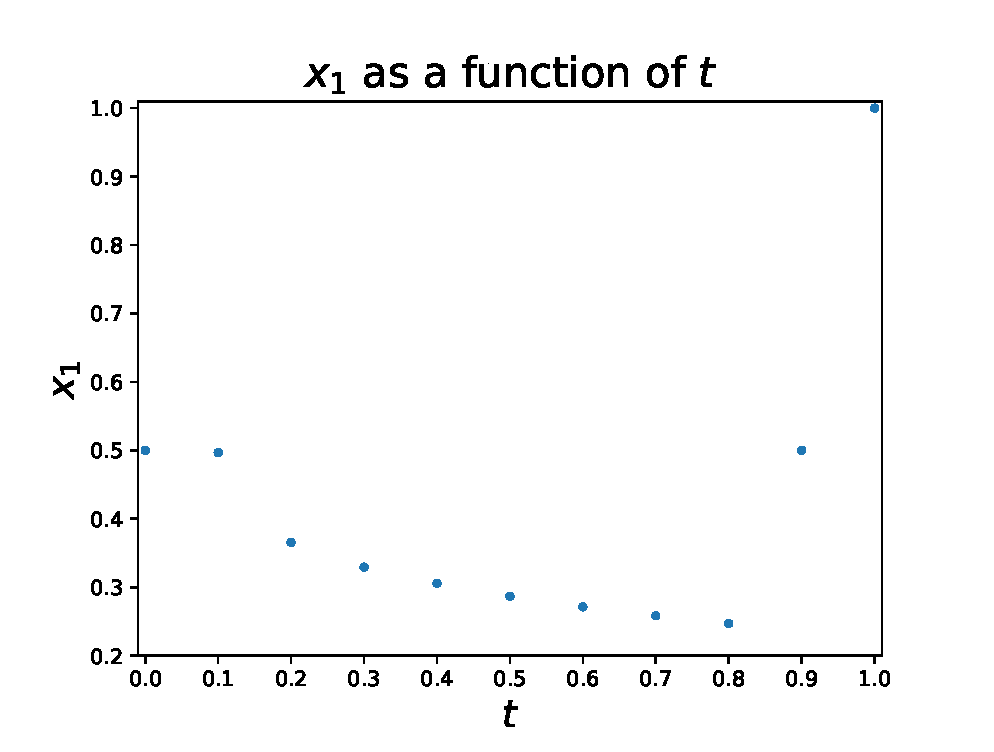
\includegraphics[scale=0.4]{x1_2}
	\caption{Illustration of how $x_1$ changes over time using the path following algorithm}
\end{figure}
\end{column}
\end{columns}
\end{frame}
\end{document}